\documentclass[12pt,a4paper]{scrartcl}

\usepackage[a4paper, left=2cm, right=1cm, bottom=1cm, top=1cm, includeheadfoot]{geometry}
\usepackage[ngerman]{babel}
\usepackage[utf8]{inputenc} % comment this if you uncomment utf8x
%\usepackage[utf8x]{inputenc} % uncomment this if there are problems with 'ä', 'ü', 'ö'
\usepackage{ucs}
\usepackage[usenames,dvipsnames]{xcolor}
\usepackage[fleqn]{amsmath}
\usepackage{amsfonts}
\usepackage{amssymb}
\usepackage{color}
\usepackage{listings}
\usepackage{hyperref}
\usepackage{amsfonts}
\usepackage{listings}
\usepackage{scrpage2}
\usepackage{graphicx}


\definecolor{mygray}{rgb}{0.9,0.9,0.9}
\lstset{language=[Visual]Basic, morekeywords={param, local}}


\lstset{
   literate={ö}{{\"o}}1
           {ä}{{\"a}}1
           {ü}{{\"u}}1
           {ß}{{\ss}}1
           {é}{{\'e}}1,
   inputencoding=ansinew,
   extendedchars=true,
   basicstyle=\scriptsize\ttfamily,
   numberstyle=\scriptsize,
   breaklines=true,
   tabsize=2,
   numbersep=5pt
}
\lstdefinestyle{customcpp}{
   language=C++,
   backgroundcolor=\color{mygray},
   numbers=left,
   keywordstyle=\color{blue}\bfseries,
   stringstyle=\color{BrickRed}\ttfamily,
   commentstyle=\color{OliveGreen}\ttfamily,
   showspaces=false,
   showstringspaces=false,
   showtabs=false
}
\lstdefinestyle{customoutput}{
   backgroundcolor=\color{mygray},
   numbers=none,
   showspaces=false,
   showtabs=false
}

\newcommand{\sourceCode}[1]{\lstinputlisting[style=customcpp]{#1}} %beinhaltet alle benötigten Packages etc.
\begin{document}
\graphicspath{{./}}

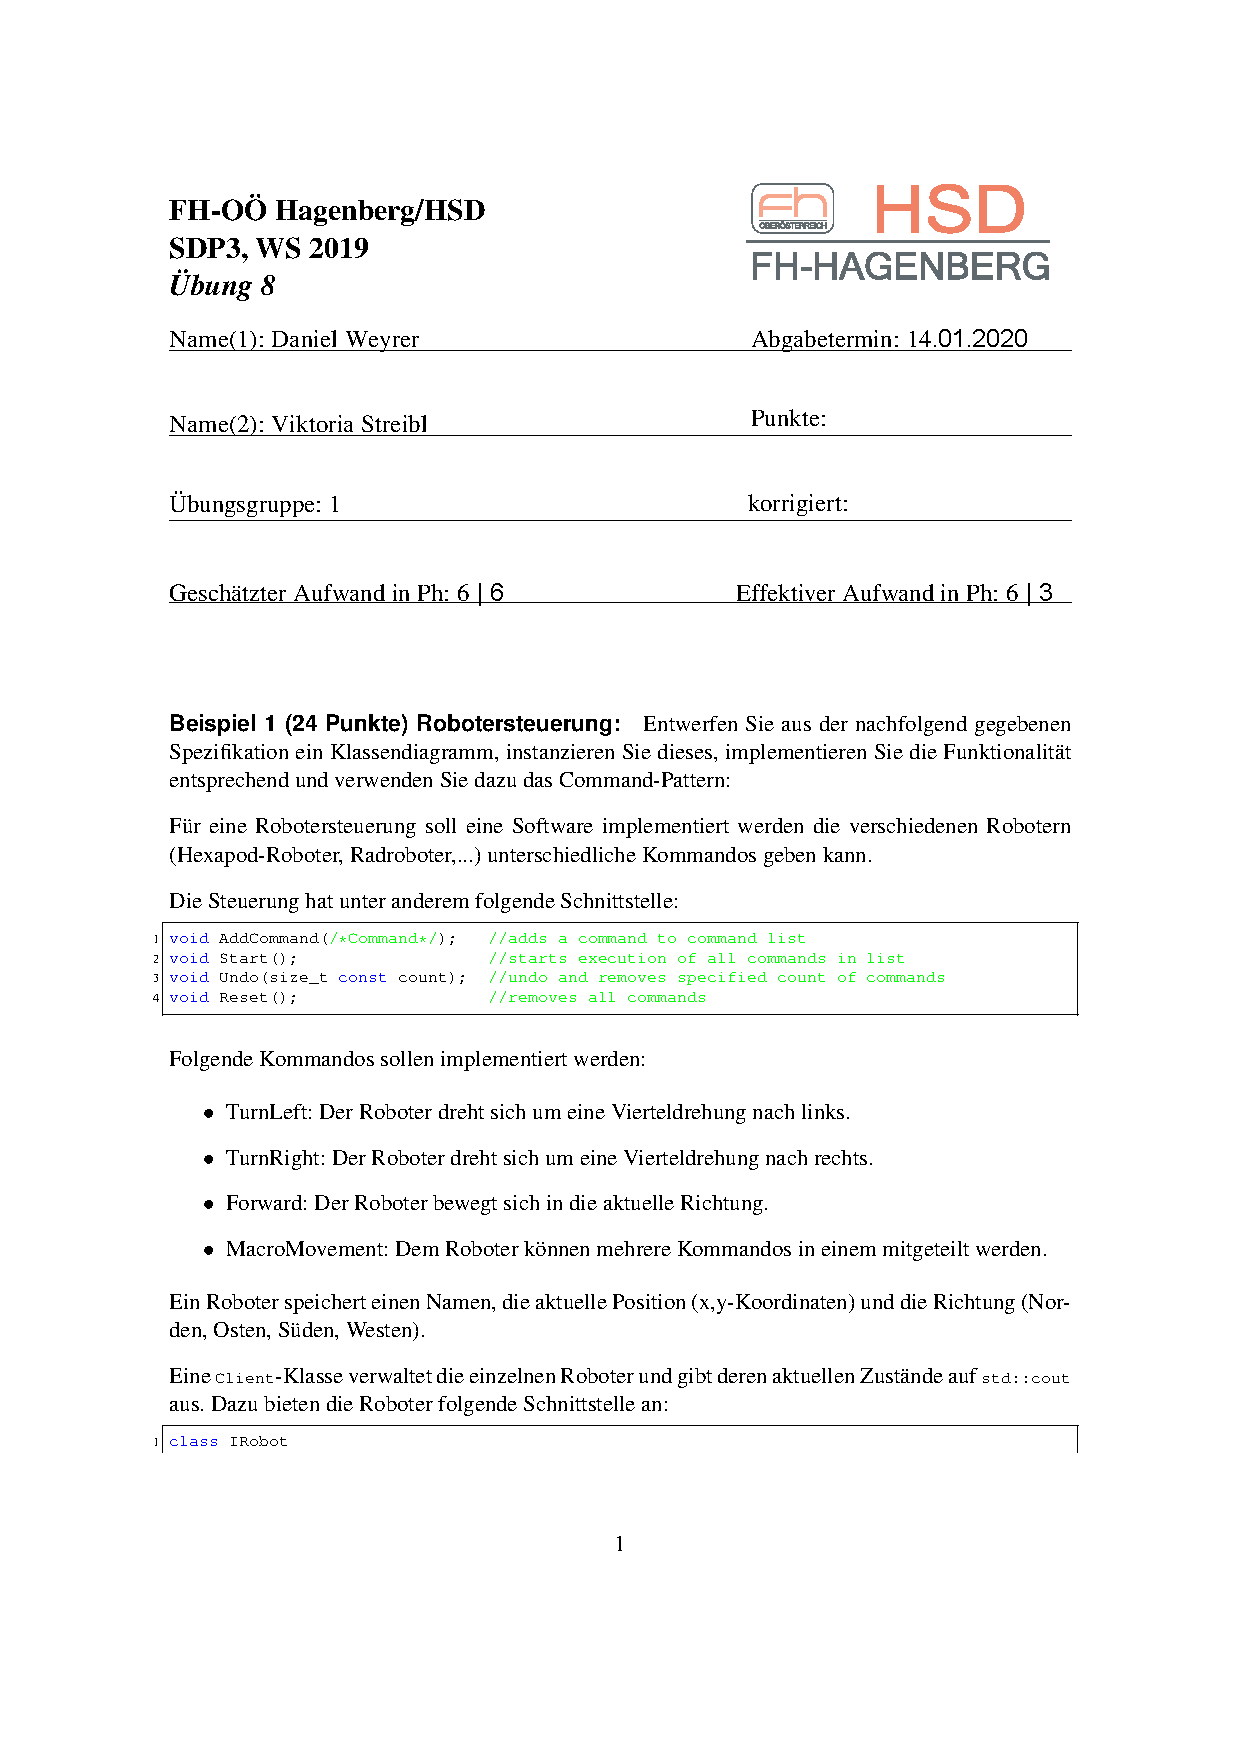
\includepdf[pages=-]{../Angabe.pdf}

\title{SDP - Exercise 08} % Übungsname und Nummer angeben
\subtitle{winter semester 2019/20} % Semester angeben oder auskommentieren, falls nicht erwünscht
\author{
Viktoria Streibl - S1810306013\\
  Daniel Weyrer - S1820306044
} % Autorenname
\date{\today} % Das heutige Datum automatisch einfügen

\maketitle % Titelseite erstellen

\newpage
\tableofcontents % Inhaltsverzeichnis erstellen
\newpage

\ihead{Viktoria Streibl}
\ohead{Daniel Weyrer}
\chead{SDP3-UE Uebung 08}

\section{Organizational}
\subsection{Team}
\begin{itemize}
	\item Viktoria 	Streibl 		- 	S1810306013
	\item Daniel 	Weyrer		-	S1820306044
\end{itemize}

\subsection{Roles and responsibilities}
\subsubsection{Jointly}
\begin{itemize}
	\item Planning
	\item Documentation
	\item Systemdocumentation
	\item Class Diagram
\end{itemize}

\subsubsection{Viktoria Streibl}
\begin{itemize}
	\item Client
	\item Hexapod
	\item IRobot
	\item Object
	\item Robot
	\item Wheelbot
	\item TestDriver
\end{itemize}

\subsubsection{Daniel Weyrer}
\begin{itemize}
	\item Control
	\item Forward
	\item ICommand
	\item MacroMovement
	\item TestDriver
	\item TurnLeft
	\item TurnRight
\end{itemize}

\subsection{Effort}

\subsubsection {Viktoria Streibl}
\begin{itemize}
	\item estimated: 6 ph 
	\item actually: 3 ph
\end{itemize}

\subsubsection {Daniel Weyrer}
\begin{itemize}
	\item estimated: 6 ph 
	\item actually: 6 ph
\end{itemize}

\section{Requirenment Definition(System Specification)}
This program should reflect robot control. Different robots should receive different commands and react accordingly.
The following commands were requested:
\begin{itemize}
	\item Turn Left
	\item Turn Right
	\item Forward
	\item MacroMovement - get multiple commands
\end{itemize}

\section{System Design}
\subsection{Design Decisions}
\subsubsection{Case-Statements in TurnLeft and TurnRight}
To make the commands independent from each other (so there`s no need to implement a TurnRight when there is a TurnLeft and the other way round), both Commands have the complete Implementation for their Undo-Command!

\newpage
\subsection{Classdiagram}
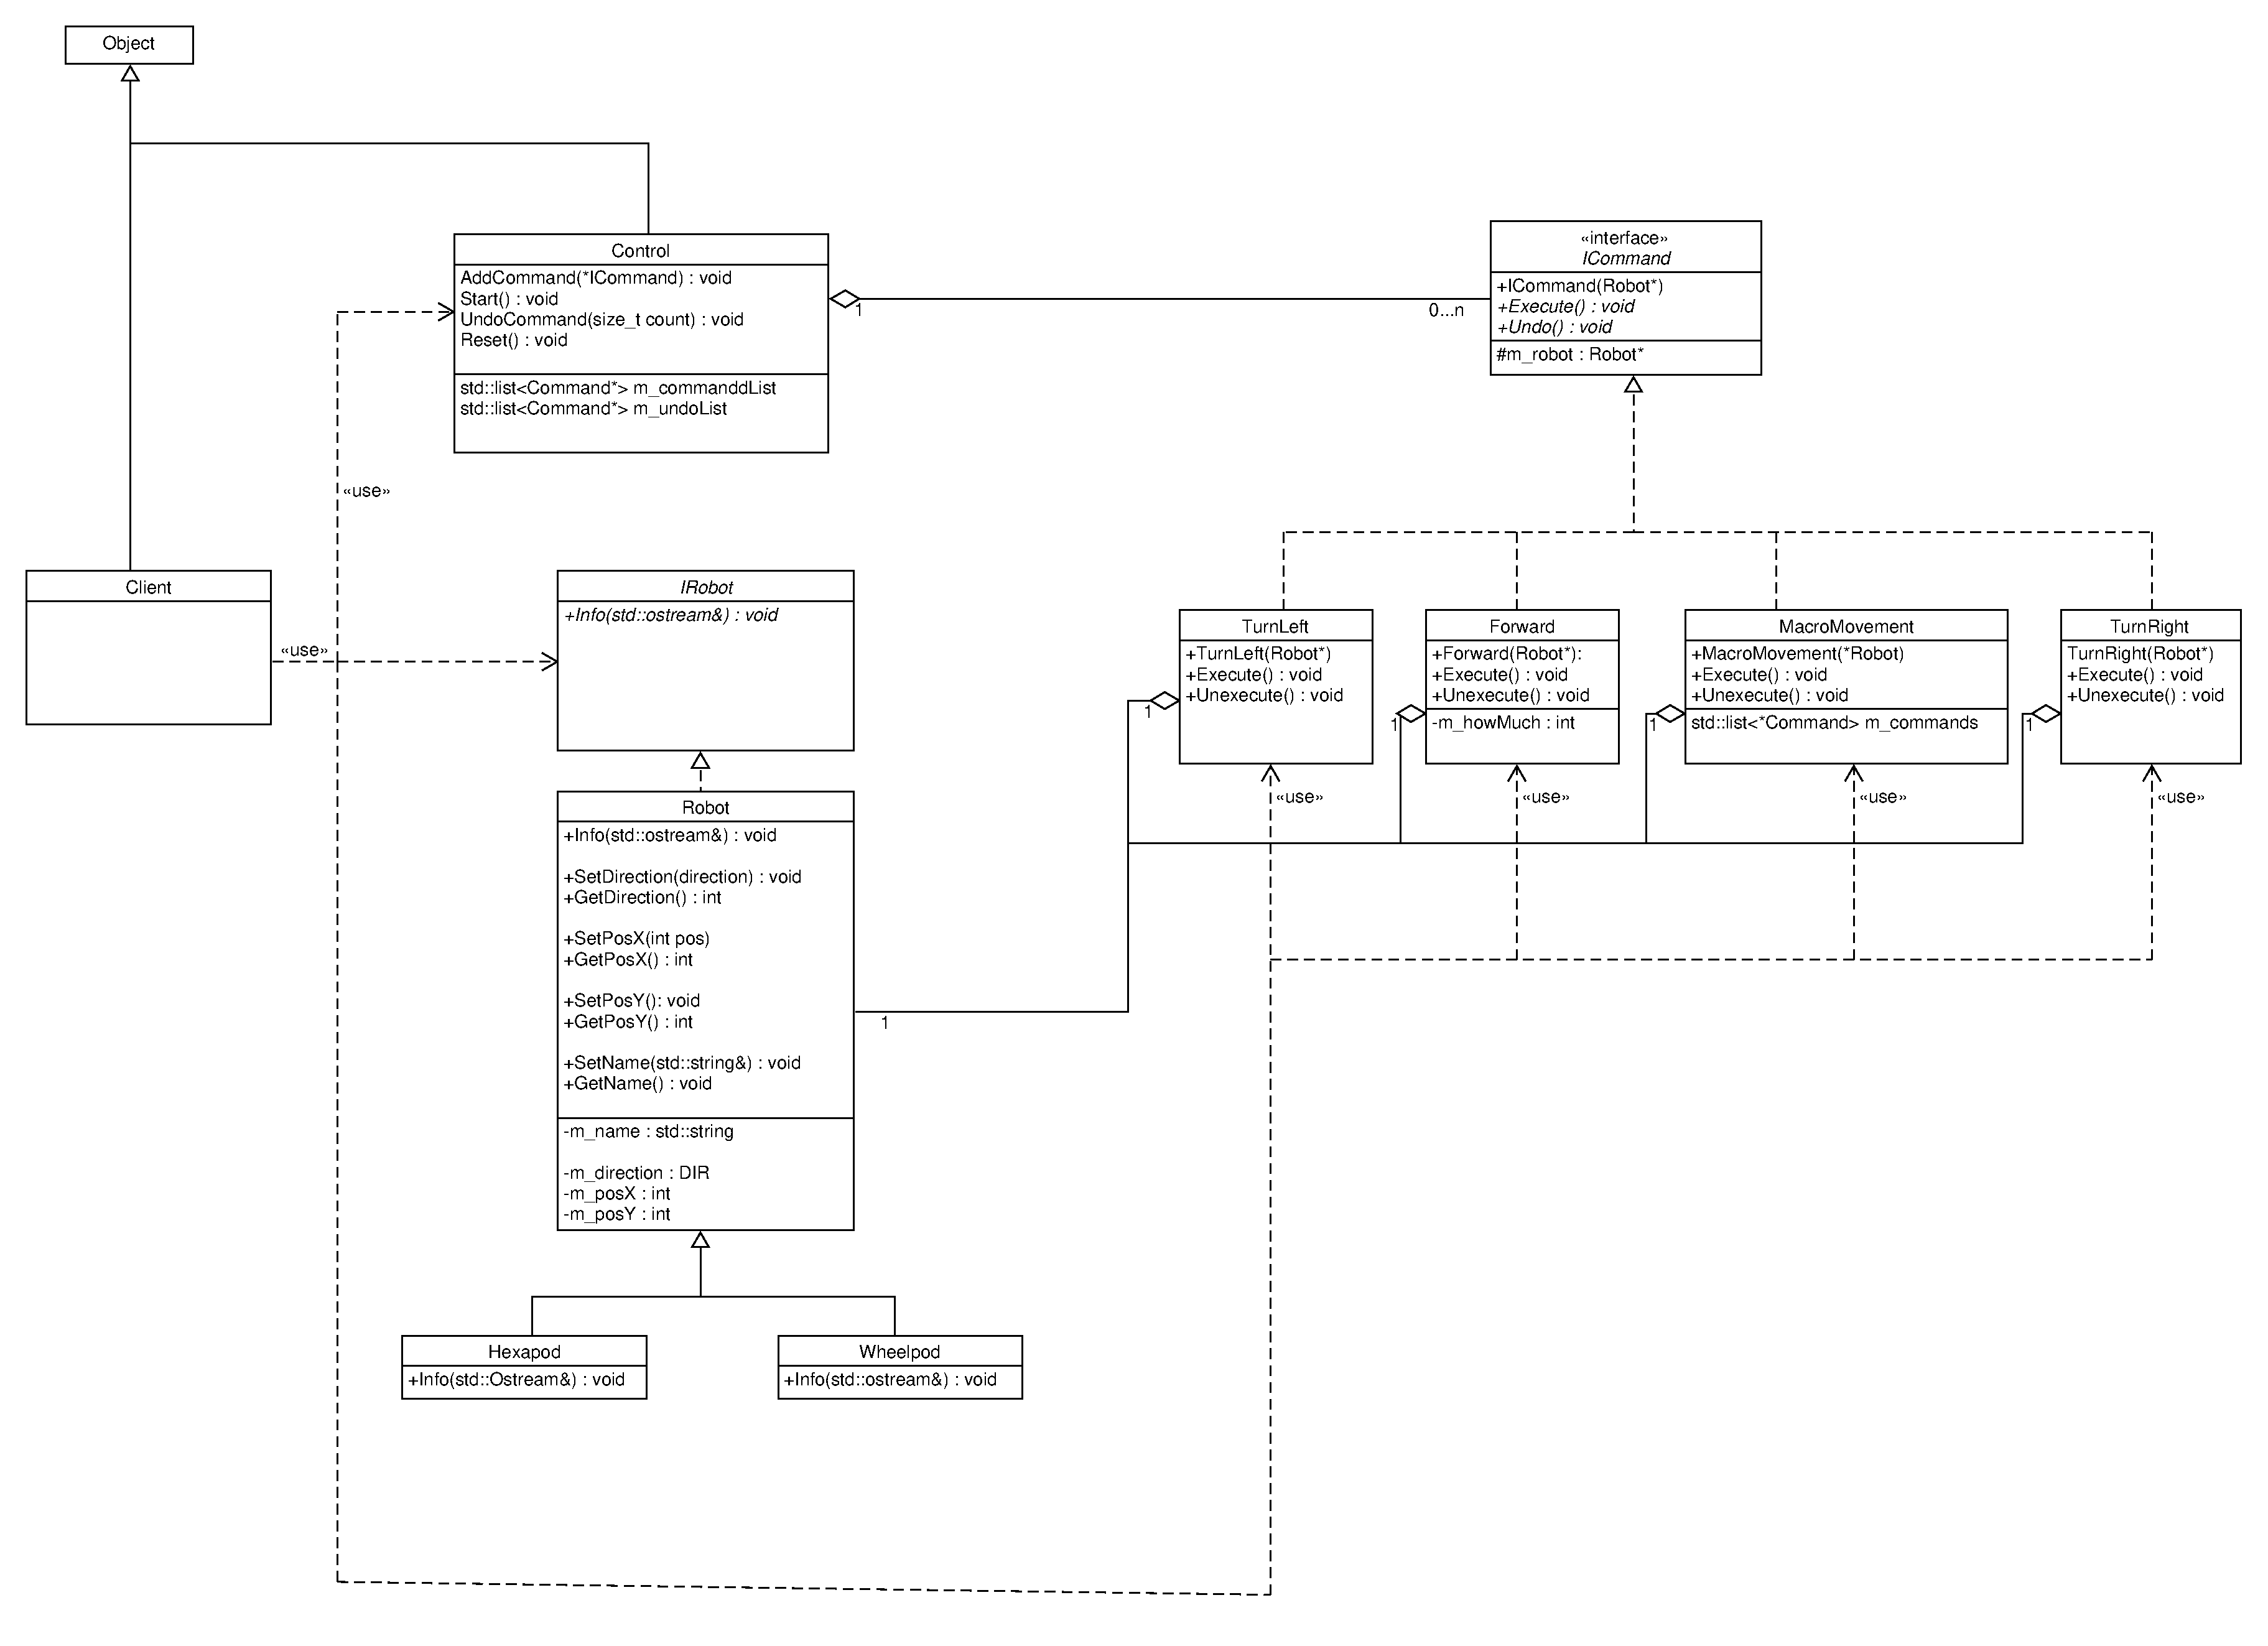
\includegraphics[scale=0.4, angle=90]{../ClassDiagram.pdf}

\section{Component Design}
\subsection{Client}
The client class has only one function which tests the robot control system. It creates two different robots, a hexapod and a wheelbot and sends them commands. It also checks for problems with nullptr as parameter for various calls.

\subsection{Control}
The Control class manages the Robots by saving all Commands to be applied on them in a vector. To undo all Commands, they are being saved in the undoList after they have been executed.
It has also following functions:
\begin{itemize}
	\item Add Comment
		\subitem This function gets a command and add it to the command list
	\item Start
		\subitem This functions execute all of the commands ins the command list
	\item Undo
		\subitem This function adds a command to the undo-list
	\item Reset
		\subitem This function removes all added commands from the command list. The commands in the Undo-List are kept to reset the Robot if needed.
\end{itemize}

\subsection{Hexapod}
This module is a robot type and inherits from the class Robot. It has an constructor which has the name of the robot as parameter and sets it via cTor-Call from Robot.
It also has a function Info, which prints all the informations of this robot.

\subsection{Wheelbot}
This module is a robot type and inherits from the class Robot. It has an constructor which has the name of the robot as parameter and sets it and sets it via cTor-Call from Robot.
It also has a function Info, which prints all the informations of this robot.

\subsection{ICommand}
This is an Interface and stores the robot, which is given via the constructor.
It declares the functions Execute() and Unexecute(). 
Used to create Pointers of this Type and Call both functions (Unexecute() reverts the Actions Execute() did)

It helds a shared pointer to the Robot the Command is meant for - to avoid code-duplication, the Constructor has been moved to this interface!

\subsection{IRobot}
IRobot is an interface. It declares the method Info with and ostream parameter to print current Location and the direction of the Robot.

\subsection{Robot}
This modul has an enum class DIR, it contains the directions north, south, east and west.
The class Robot inherits from the Interface IRobot. It stores the name, direction, x-, and y-position.
It also implements the following Get-/Setmethods:
\begin{itemize}
	\item Set/Get-Direction
	\subitem The setter gets a direction and saves it. The getter returns the stored direction of the robot.
	\item Set/Get-PosX
	\subitem The setter gets the x-position and saves it. The getter returns the stored direction of the robot.
	\item Set/Get-PosY
	\subitem The setter gets the y-position and saves it. The getter returns the stored direction of the robot.
	\item Set/Get-Name
	\subitem The setter gets the name of the robot and saves it. The getter returns the stored direction of the robot.
\end{itemize}

\subsection{Forward}
It overrides the functions Execute and Unexecute.  These functions increase or decrease the position x,y depending on the direction.

\subsection{TurnLeft}
Changes the direction of the Robot by 90 degrees clockwise.

\subsection{TurnRight}
Changes the direction of the Robot by 90 degrees counter-clockwise.

\subsection{MacroMovement}
Takes a vector of shared pointers of commands. When calling the function Execute(), all Commands in the vector are being Execute one by one and stored in the undo-list, to revert all the changes it did.

\section{Source Code}

\subsection{Client}
\subsubsection{Client.h}
\sourceCode{../../Robot/Robot/Client.h}
\subsubsection{Client.cpp} 
\sourceCode{../../Robot/Robot/Client.cpp}
\newpage

\subsection{Control}
\subsubsection{Control.h}
\sourceCode{../../Robot/Robot/Control.h}
\subsubsection{Control.cpp}
\sourceCode{../../Robot/Robot/Control.cpp}
\newpage

\subsection{Hexapod}
\subsubsection{Hexapod.h}
\sourceCode{../../Robot/Robot/Hexapod.h}
\subsubsection{Hexapod.cpp}
\sourceCode{../../Robot/Robot/Hexapod.cpp}
\newpage

\subsection{Wheelbot}
\subsubsection{Wheelbot.h}
\sourceCode{../../Robot/Robot/Wheelbot.h}
\subsubsection{Wheelbot.cpp}
\sourceCode{../../Robot/Robot/Wheelbot.cpp}
\newpage

\subsection{ICommand}
\subsubsection{ICommand.h}
\sourceCode{../../Robot/Robot/ICommand.h}
\subsubsection{ICommand.cpp}
\sourceCode{../../Robot/Robot/ICommand.cpp}
\newpage

\subsection{IRobot}
\subsubsection{IRobot.h}
\sourceCode{../../Robot/Robot/IRobot.h}
\subsubsection{IRobot.cpp}
\sourceCode{../../Robot/Robot/IRobot.cpp}
\newpage

\subsection{Robot}
\subsubsection{Robot.h}
\sourceCode{../../Robot/Robot/Robot.h}
\subsubsection{Robot.cpp}
\sourceCode{../../Robot/Robot/Robot.cpp}
\newpage

\subsection{Forward}
\subsubsection{Forward.h}
\sourceCode{../../Robot/Robot/Forward.h}
\subsubsection{Forward.cpp}
\sourceCode{../../Robot/Robot/Forward.cpp}
\newpage

\subsection{TurnLeft}
\subsubsection{TurnLeft.h}
\sourceCode{../../Robot/Robot/TurnLeft.h}
\subsubsection{TurnLeft.cpp}
\sourceCode{../../Robot/Robot/TurnLeft.cpp}
\newpage

\subsection{TurnRight}
\subsubsection{TurnRight.h}
\sourceCode{../../Robot/Robot/TurnRight.h}
\subsubsection{TurnRight.cpp}
\sourceCode{../../Robot/Robot/TurnRight.cpp}
\newpage

\subsection{MacroMovement}
\subsubsection{MacroMovement.h}
\sourceCode{../../Robot/Robot/MacroMovement.h}
\subsubsection{MacroMovement.cpp}
\sourceCode{../../Robot/Robot/MacroMovement.cpp}
\newpage

\subsection{Object}
\subsubsection{Object.h}
\sourceCode{../../Robot/Robot/Object.h}
\newpage

\subsection{TestDriver}
\subsubsection{TestDriver.cpp}
\sourceCode{../../Robot/Robot/TestDriver.cpp}

\subsection{output}
\sourceCode{../../Robot/Robot/test.txt}

\newpage


\end{document}